\documentclass{article}
\usepackage[T1]{fontenc}
\usepackage{lmodern}
\usepackage{graphicx}
\usepackage{amsmath,amssymb}
\usepackage[a4paper,margin=2cm]{geometry}
\usepackage[absolute,overlay]{textpos}
\setlength{\TPHorizModule}{1mm}
\setlength{\TPVertModule}{1mm}
\usepackage[indonesian]{babel}
\usepackage{hyperref}
\setlength{\emergencystretch}{2em}
% unit: Halaman 83

\begin{document}

% === Halaman 83 (llm) ===

\vspace{53.46mm}

\section*{Struktur file audio WAV}

\vspace{10mm}

% deskripsi: Diagram struktur format file WAVE yang mencakup deskriptor chunk RIFF, sub-chunk fmt, dan sub-chunk data, lengkap dengan offset file dan ukuran field.
% bbox normalisasi: [0.0200, 0.1200, 0.4200, 0.8900]
\begin{textblock*}{84.00mm}(4.20mm,35.64mm)
\noindent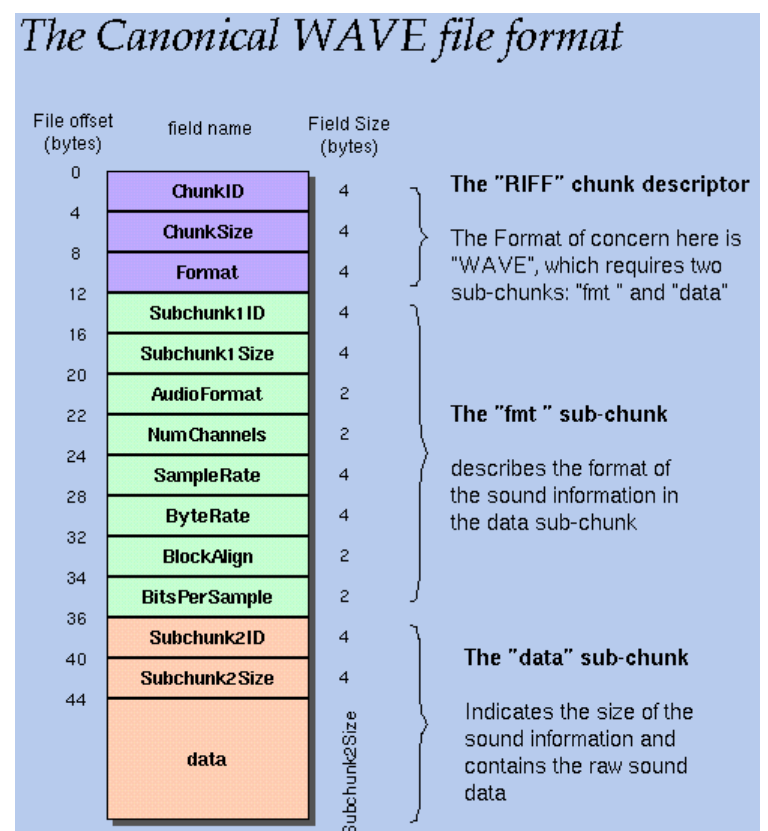
\includegraphics[width=84.00mm,height=228.69mm]{../../images/llm/page_083_img_01.png}%
\end{textblock*}

% deskripsi: Ilustrasi struktur frame audio WAV yang menunjukkan header (Encoding, Channels, Frame Rate, Bit Depth) dan sampel data audio untuk beberapa frame (Frame #1, Frame #2, Frame #N).
% bbox normalisasi: [0.4400, 0.1200, 0.9900, 0.3000]
\begin{textblock*}{115.50mm}(92.40mm,35.64mm)
\noindent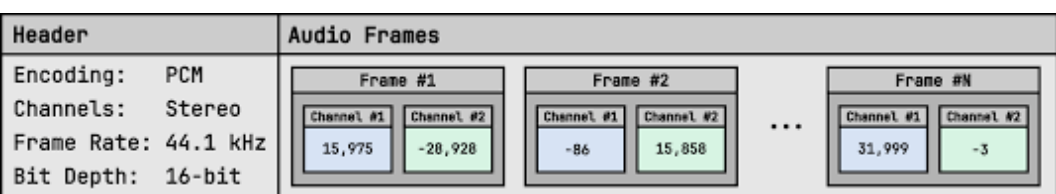
\includegraphics[width=115.50mm,height=53.46mm]{../../images/llm/page_083_img_02.png}%
\end{textblock*}

\end{document}
